\chapter{Computational Model} \label{model}

\newcommand{\numcategories}[0]{$cat$ }
\newcommand{\numsubcategories}[0]{$cat$ }
\newcommand{\numsensors}[0]{$N_S$ }
\newcommand{\numstakeholders}[0]{$N_{DC}$ }
\newcommand{\numcontexts}[0]{$N_C$ }
\newcommand{\numquestions}[0]{$N_{DR}$ } 
\newcommand{\numsubfeatures}[0]{$num_{sf}$ } 




\section{Introduction}
The aim is to create a computational model that is able to collect useful information about the influence of monetary incentives on mobile
data sharing. (Quote some studies that have done similar studies with no data incentives). 
The users are first asked some preliminary questions to form a profile about them. The model proceeds to use the user profiles 
formed to assign each sensor data request
with a maximum achievable credit. The model attempts identifies the data requests where users might not be inclined to share mobile sensor data willingly. These data requests are assigned higher maximum obtainable costs. Similarly, the data requests where the users would want to share more mobile sensor data
is assigned a lower maximum obtainable cost. This permits us to see whether incentives do indeed make a difference in mobile sensor
data sharing. The model aims to identify the amount of data each user would share for a data request and assign maximum obtainable costs accordingly.

\section{Model Intricacies}

\begin{figure}[ht!]
\centering
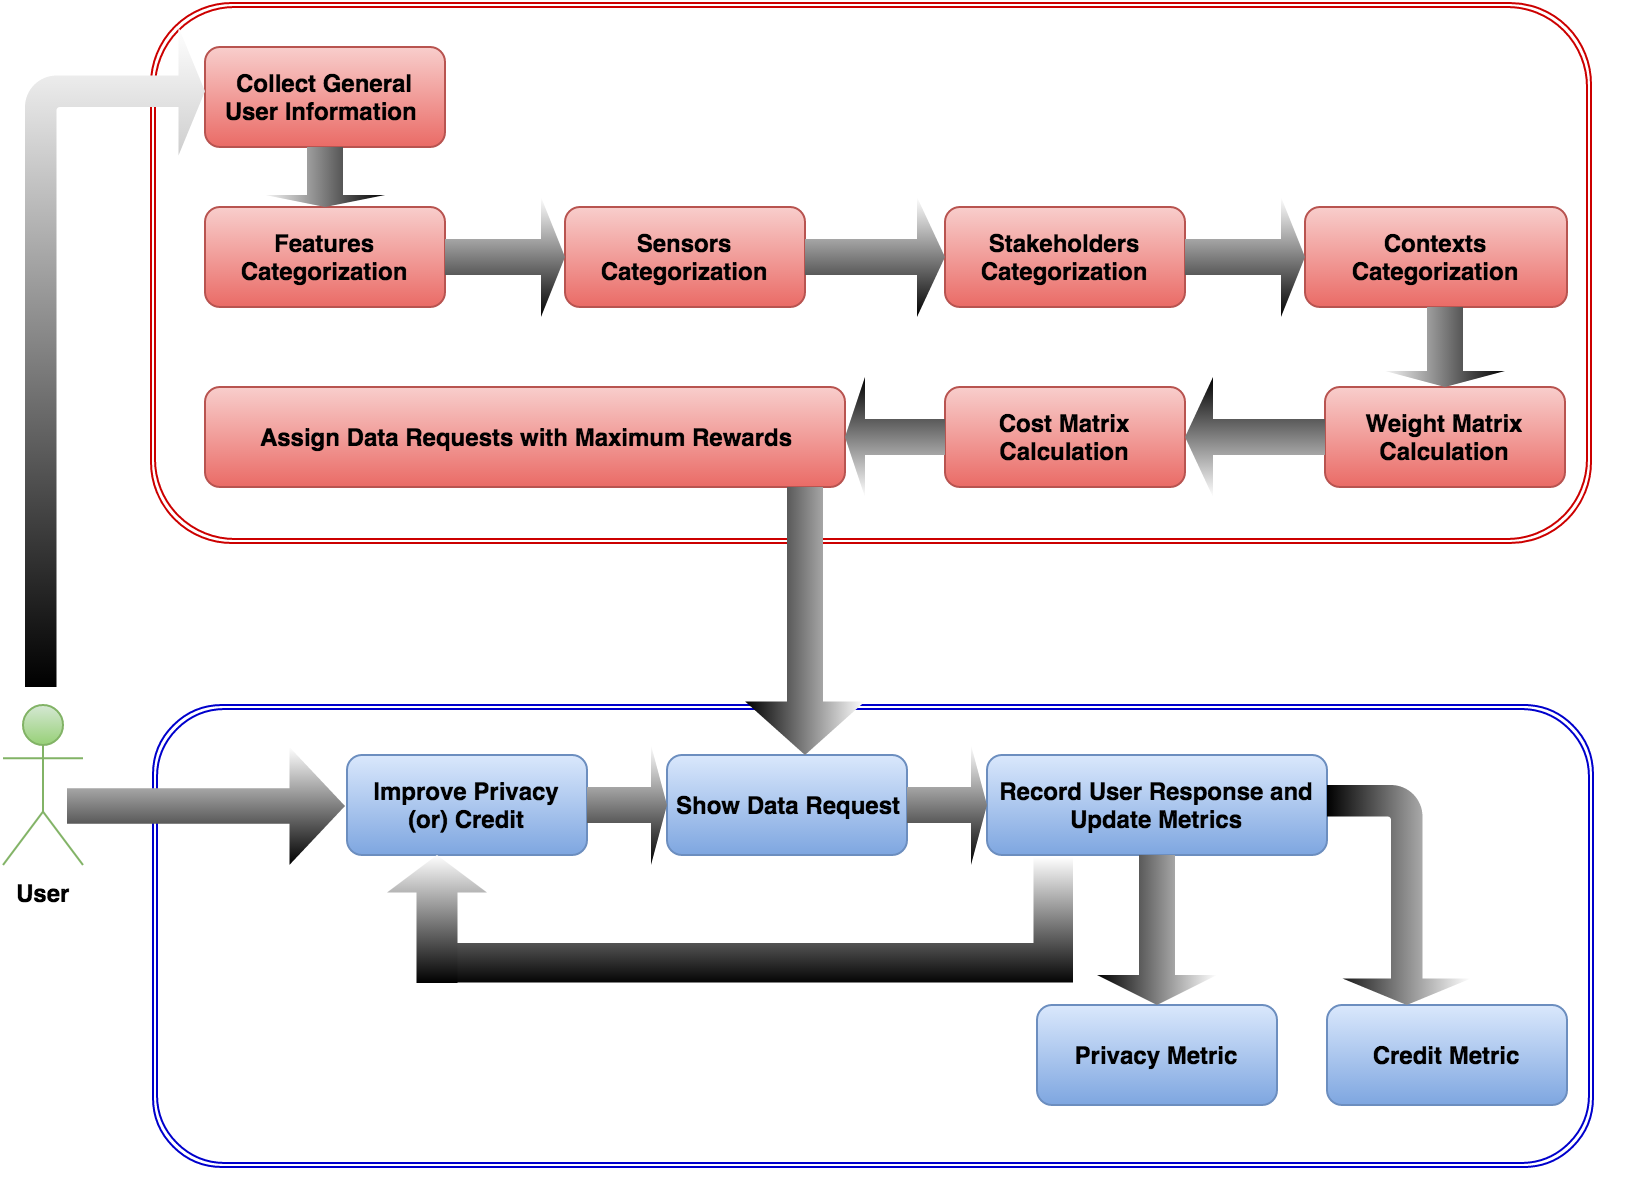
\includegraphics[width=\textwidth,keepaspectratio]{./images/model_building_blocks}
\caption{Computational Model Flow Chart \label{model_blocks}}
\end{figure}

The sections below explain the various building blocks of the computational model. The Figure \ref{model_blocks}
provides an overview of the flow of the model.

\subsection{Collecting User Information}
To begin with the model, each user is asked to enter various non-intrusive personal information. The information collected can consist of but is not limited to :

\begin{itemize}
\item Gender
\item Year of birth
\item Country
\item Education Level
\item Occupation
\item Frequency of mobile phone use per day
\item List of different mobile applications present on the users phones
\end{itemize}

Collecting this information is crucial to the data analysis that is conducted in the later stages.
\subsection{Categorization of the Features} \label{catfeatures}
After the users personal information is collected, users are asked to place the features in categories according to how privacy intrusive they are to the user. A feature can be one of the following:

\begin{itemize}
\item \textbf{Sensors} : Sensors consist of the sensors in the mobile phone which users
can trade in a data request
\item \textbf{Stakeholders} : Stakeholders
consist of any entity that can request the user for mobile sensor data
\item \textbf{Contexts} : Contexts consist of the purpose for which a Stakeholder would like to obtain the user's mobile sensor data
\end{itemize}

Features are the three dimensions that form a unique data request. A data request is defined as a Stakeholder asking users to share their mobile Sensor data for a particular Context.

As mentioned before, users are asked to categorize the features into one of the five categories:

\begin{enumerate}
\item Very low privacy intrusion
\item Low privacy intrusion
\item Medium privacy intrusion
\item High privacy intrusion
\item Very high privacy intrusion
\end{enumerate}

Categories are linearly scaled and equally spaced. As indicated by the numbers on the left of the categories, these range from one to five and users can place each of the Features in a category according to their perceived intrusion level. Category one represents that the Feature does not contribute a lot to the data sharing decision. Similarly, category five represents that the Feature  contributes a lot to the user's data sharing decision. Similarly, categorfive represents that users are reluctant to give away their sensor data for this feature. More than one feature can be placed in the same category, which makes it a more powerful tool than the ranking mechanism.

Let the variable \numcategories represent the number of categories, which here is five. Additionally, let the category assigned to the Sensors be represented by the variable $se$, the category assigned to the Stakeholders be represented by the variable $st$ and the category assigned to the Contexts be represented by the variable $co$.

Once users have categorized the Sensors, Stakeholders and the Contexts into the respective categories reflecting the importance of each of the features in the data sharing decision, each feature is assigned a weight.
Let the respective weights of Sensors, Stakeholders and Contexts be represented by the variables, $w_{se}$, $w_{dc}$ and $w_{co}$ are calculated as follows :

\begin{equation}
   w_{se} = \frac{se}{se+st+co} 
\end{equation}
\begin{equation}
   w_{st} = \frac{st}{se+st+co}  
\end{equation}
\begin{equation}
   w_{co} = \frac{co}{se+st+co}  
\end{equation}


\subsection{Categorization of the Sub-Features}
Once the features have been categorized and their weights calculated as above, sub-features are to be categorized. A sub-feature
is defined as one type of a feature. In other words, sub-features are the different types of features that appear during data request to the user. The following are examples of sub-features for each feature :

\begin{itemize}
\item Sensors : 
\begin{itemize}
\item Accelerometer
\item  Battery
\item Gyroscope
\end{itemize} 
\item Stakeholders : 
\begin{itemize}
\item Corporation
\item  Government
\item Educational Institution
\end{itemize}
\item Contexts :
\begin{itemize}
\item Education
\item Navigation
\item Gaming
\end{itemize}
\end{itemize}

\begin{figure}[ht!]
\centering
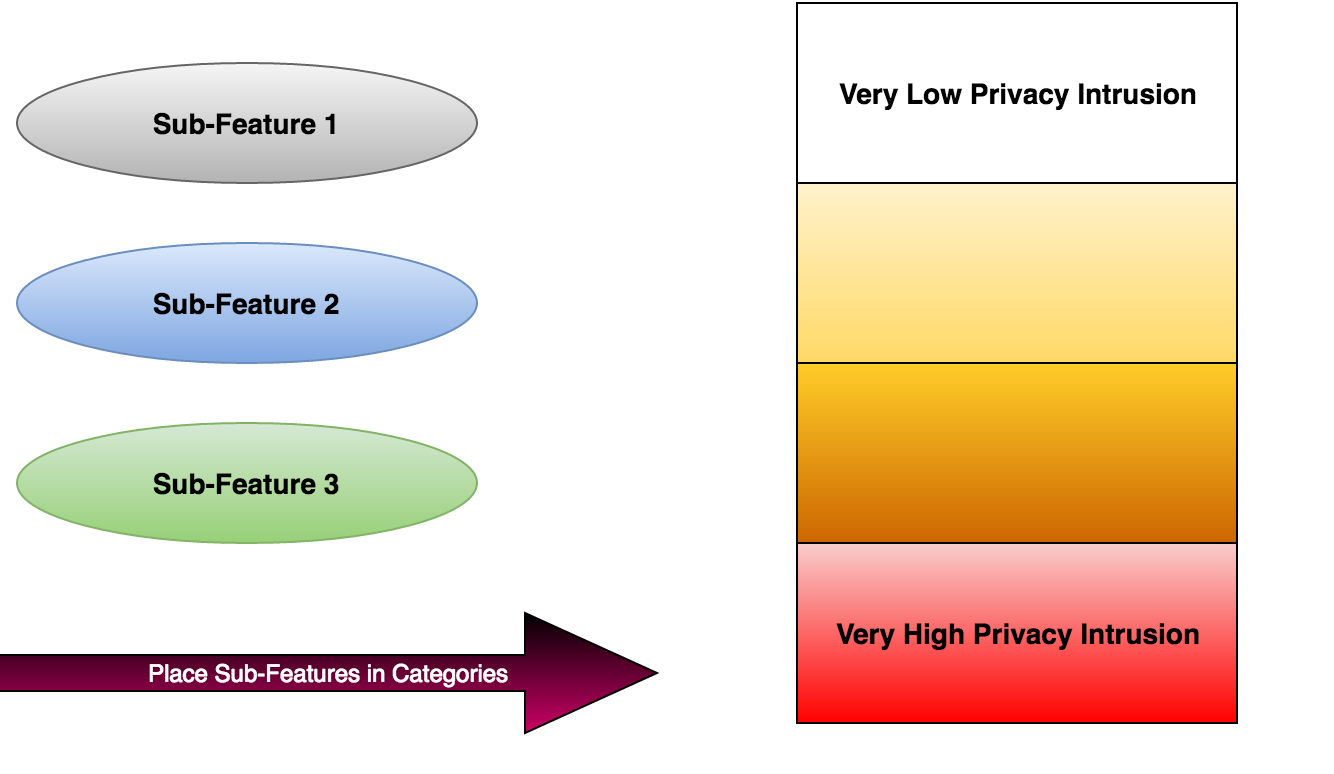
\includegraphics[width=\textwidth,keepaspectratio]{./images/categorize_sub}
\caption{Categorizing Sub-Features according to the perceived Intrusion Level \label{categorize_sub}}
\end{figure}

Each of the above are different kinds or sub-features of the respective Features. 
For each of the available features, the respective sub-features need to be in turn categorized in a similar fashion to section \ref{catfeatures}.
The categories are the same as mentioned in the previous section. Let \numsubfeatures be the number of sub-features each feature has.


The first category indicates that users find the sub-feature would not hinder the data sharing decision. This means that the user would not be worried trading data for a data request involving this sub-feature. The last category indicates that users find this sub-feature would hinder the data sharing decision . This means that users would be reluctant of giving data for a data request involving this sub-feature. As seen in the conceptual diagram is shown in figure \ref{categorize_sub}, users place each of the sub-features available for every feature in the given categories.

Let every sub-feature be represented by a unique identifier within its feature. For example, in the list of sub features provided above, accelerometer is the first sub-feature of sensors, corporation is the first sub-feature of stakeholders and education is the first sub-feature of contexts. For each of the sub-features of Sensors, categories they are placed in by users is represented by $se_{i}$ and $i$ is the identifier
of the sub-feature. Similarly, categories assigned to sub features of features Stakeholders and Contexts respectively are represented by $st_{j}$ and $co_{k}$, where $j$ and $k$ are the identifiers of the sub-features categorized.

\subsection{Weight Matrix Calculation}
Each data request to users consists of the three above mentioned features in them. Each of the features each have \numsubfeatures sub-features that can appear in turns in a data request. So the total number of data requests are :

\begin{equation}
num_{dr} =  num_{sf} * num_{sf} * num_{sf}   
\end{equation}

Let $WM$  be a matrix with three dimensions $num_{sf} x num_{sf} x num_{sf} $. We call this the weight matrix.
Each cell of $WM$, that is $WM_{i,j,k}$ represents a data request which involves the Sensors sub-feature with identifier $i$, Stakeholders sub-feature with identifier $j$,
and the Contexts sub-feature with identifier $k$. That is, each cell of $WM$ represents the weight of a data request to the users. The aim of the weight matrix is to use the information collected from the user categorizations, to assign weights to each data requests. Intuitively, the process examines the
data requests where the user is least likely to trade data and assigns higher weights to those data requests. This process can be seen in
section \ref{analysis_model} with examples. As mentioned before, each cell of the matrix $WM$ represents the weight of a data request with a unique Sensors sub-feature $i$, Stakeholders sub-feature $j$ and Contexts sub-feature $k$. To calculate the weight of a data request :

\begin{equation}
WM_{i,j,k} = (se*se_{i}) + (st*st_{j}) + (co*co_{k})
\end{equation}

Applying this formula for every possible values of $i$, $j$ and $k$ gives the weight matrix $WM$.

\subsection{Cost Matrix Calculation}

Once $WM$ has been calculated, it can give an idea of the weight each data request receives. The aim is now to assign a maximum obtainable cost to each data request. This cost is the maximum credit users can receive for a particular data request. Let $CM$ be the cost matrix with the three dimensions $num_{sf} x num_{sf} x num_{sf} $.
Let it be assumed to have a budget of $b$ for a day, where
$b$ can be in an actual currency or any sorts of virtual credits. In this literature the budget will be referred to with the unit credits. Each cell of the cost matrix will represent the amount of credits allocated for a particular data request for one day.
To begin with, we calculate the sum of all the cells of the weight matrix $WM$:

\begin{equation}
sum_{WM} = \sum\limits_{i=1}^{num_{sf}} \sum\limits_{j=1}^{num_{sf}} \sum\limits_{k=1}^{num_{sf}} wm_{i,j,k}
\end{equation}

where the function $sum_{WM}$ gives the sum of a matrix, in this case the weight matrix.
Let $CM_{i,j,k}$ represent the credit allocated for the data request which involves the Sensor's sub-feature with identifier $i$, Stakeholder's sub-feature with identifier $j$, and the Context's sub-feature with identifier $k$. To calculate one cell of the cost matrix :

\begin{equation}
CM_{i,j,k} = \frac{WM_{i,j,k} * b}{sum_{WM}}
\end{equation}

Repeating the above for every cell of $CM$, the entire cost matrix can be calculated. Now, all the maximum obtainable costs have been allocated per day for every data request.

\subsection{Cost and Privacy Metrics} \label{o}
Every data request has been assigned a cost. This is the maximum cost that a user can obtain for that data request.
The Cost metric is the total amount of credits the user has obtained by trading data for data requests for one day. Similarly, the Privacy metric is the amount of privacy percentage obtained while trading data for requests. It intuitively quantifies the amount of data the user has refused to share hence implying privacy. The Cost and Privacy metrics are inversely proportional to each other, in the sense that when the Cost increases the Privacy decreases and vice versa.

Each data request the user chooses how much data is to be shared, from the maximum amount of data to no data at all. The possible responses to a data request are called options. Each option corresponds to a summarization level explained in detail in section \ref{summa}. The cost assignment to each option is linearly scaled according
to the cost assigned to each data request. Let us assume there are options for a data request ranging from $1$ to $m$ (numeric options), where $1$ corresponds to the option where the users give all their data for a request and $m$ to where the users choose not give any data for a request. Therefore there are a total of $m$ options for every data request. For each option in a data request is associated with:

\begin{itemize}
\item The amount of credit change from this particular option for a data request
\item The amount of privacy change from this particular option for a data request
\end{itemize}

While assigning costs to data requests there are two scenarios to consider:

\begin{itemize}
\item Assigning option costs without a participation cost. Users are not rewarded for their participation
\item Assigning option costs inclusive of a participation cost. Users are rewarded for responding to data requests irrespective of how much data they choose to share
\end{itemize}

Let us examine the first scenario. Let the option costs be calculated for the data request with Sensors sub-feature $i$, stakeholders sub-feature $j$ and
contexts sub-feature $k$. The assigned cost for any option numbered $h$ of this data request is calculated as follows:

\begin{equation}
cost_{h} =  \frac{CM_{i,j,k}*(m-h)}{m-1}
\end{equation}

Applying this formula by replacing $h$ by the option numbers from $1$ to $m$ gives the cost the user can receive for each option.


Similarly, if a participation cost would like to be assigned to each option, it would mean that even tough the user does not share data, they still
receive some credit for answering the data request. This concept can be implemented to ensure user participation in the experiment. (Quote some paper with
participation of users in PSS). Let $x$ be a fraction of the total budget $b$ that is dedicated for user participation. Using a geometric progression with $a=1$ and $r=\sqrt[(m-1)]{x}$ , we can calculate the fraction of the maximum cost obtainable from a data request $frac_{h}$, an option numbered $h$ gets:

\begin{equation}
frac_{h} = a * r^{h-1}
\end{equation}

The fraction of the cost an option $h$ can be assigned has been calculated, to get the cost $cost_{h}$ of option $h$ for the data request with Sensors sub-feature $i$, stakeholders sub-feature $j$ and
contexts sub-feature $k$ :

\begin{equation}
cost_{h} = frac_{h} * CM_{i,j,k}
\end{equation}
This assigns costs to each option, taking into consideration a participation cost that the user gets even if data is not shared for that data request.

Privacy percentage $pri_{h}$ is linearly scaled between the first to the $mth$ option between $0$\% and $100$\% as follows:
\begin{equation}
pri_{h} = \frac{(h-1) * 100}{m-1}
\end{equation}

The total cost and privacy is the sum and arithmetic average of all the costs and privacy respectively, obtained from every answered data request. If a data request is left unanswered, a maximum privacy of 100\% and minimum cost of 0 credit is assumed.


\subsection{Improving the Metrics}
Before users answers a question, it is useful to know what the user interest lies in. Would the user like to improve
the privacy metric, or would the user would like to increase the credit revenue. In addition, if we know what the user is looking to improve, we can retrieve the question that can improve the that particular metric the most.
For example if the user wishes to improve his privacy further, we look at the questions where the user has given the most amount of data. We then put forth this question to answer, which indicating all the options that can improve the privacy. Similarly, if the user chooses to obtain more credit, the question where the user has given least amount of data is retrieved. Options that can improve the user credit are also indicated.


\subsection{Summarization of Collected Data} \label{summa}
Each data request can have options $m$ number of options the user can choose from for every data request. These options range from $1$, which indicates that the user would like to give all his data, to option number $m$, which indicates when the user does not want to give any data to this data request. Even tough all data is encrypted these days, it is still not enough as encryptions might be cracked. Summarization is a privacy algorithms that aggregates data to provide less information than in its original form. The higher the summarization level gives less data than than in its original form. The lower the summarization level gives data closer to its original form. In this model, sensor data is collected for a period of 24 hours every $y$ seconds for every data request. If the data is summarized, according to the option chosen, the data is collected either every $y$ seconds or lesser.

Data is collected for the 24 hour period, and at the end of this period according to the option chosen by the user, it is summarized. Summarization can
be linearly assigned to each option.
The highest privacy option $m$ corresponds to the highest summarization level. The first option corresponds to the lowest summarization level. An example of assigning the summarization level $summ_{h}$ for an option h for a data request can be the following :
\begin{equation}
summ_{h} = y*h \text{ where } h \neq m
\end{equation}

This gives the frequency of sensor data collection for every option of a data request.

\section{Analysis of the Model} \label{analysis_model}
In this section, three different examples are explained in order to test some of the properties that the model assigns to the 
weight and cost matrix.

\subsection{Setup}
In the following examples, the following features and sub-feature are considered:

\begin{enumerate}
    \item Sensors
    \begin{enumerate}
    \item Accelerometer 
    \item Noise 
    \item Location 
   \end{enumerate}
    \item Stakeholders 
    \begin{enumerate}
    \item Corporation 
    \item Government 
    \item Educational Institution 
   \end{enumerate}
   \item Contexts
    \begin{enumerate}
    \item Navigation 
    \item Environment 
    \item Social Media 
   \end{enumerate}
 \end{enumerate}
 
The numbers indicated to the left of the sub-features is the sub-feature unique identifier. This uniquely identifies a sub-feature of a feature. There are in total $num_{sf}=3$ sub-features for each feature.
Each user will receive a number of $$num_{sf}*num_{sf}*num_{sf}=27$$ data requests in total. The number of categories available to categorize is $cat=5$ as explained in \ref{catfeatures}. Additionally, it is assumed that a budget $b=100$ per day is available. 
The input to the model are the user choices during the categorization of the features and sub-features.

\subsection{Results}

To begin with, the way the user has categorized the features and sub-features is introduced. This will be followed by an explanation
of the generated matrices. To make reference easier to the graphs, instead of sub-feature names, numeric identifiers are used. From now on each feature and sub-feature will be referred to by its identifier such as feature 1 for Sensors and sub-feature 2 of feature 1 for the noise sensor. The tuple (a,b,c) represents a data request with:
\begin{enumerate}
    \item a - Sensor's sub-feature a
    \item b - Stakeholder's sub-feature b
    \item c - Context's sub-feature c
   \end{enumerate}
where a, b and c are all numbers from one to three.

\subsubsection{Scenario One}

If features and sub-features have all been given the same categories respectively by users, then all data requests should be assigned equal weights and costs.
In scenario 1, the users choose categories for the Features and sub-features as shown in the table \ref{tab:scenario11}. As it can be seen in the table, each feature receives the 
category 1, and all their sub-features are categorized as 3. In short, all the features have the same categorization and their respective
sub-features all have the same categorization as well. From this input, the formulation of the weight matrix can be seen in figure \ref{weight11}, and the cost matrix can be seen in figure \ref{cost11}.
For each data request indicated as a tuple of (sensors, stakeholders, contexts) in the x-axis of figures \ref{fig:scenatio11}, all have identical weights and costs. This is due to the fact that the users find all the features and sub-features equally intrusive so all the data requests are weighted equally.

\begin{table}[h!]
  \centering
  \caption{Categorization for Scenario 1}
  \label{tab:scenario11}
  \begin{tabular}{cccc}
    \toprule
    Feature & Sub-Feature ID = 1 & Sub-Feature ID = 2 & Sub-Feature ID = 3\\
    \midrule
    Sensors & Accelerometer & Noise & Location\\
     1 & 3 & 3 & 3\\ \hhline{====}
     Stakeholders & Corporation & Government & Educational Institution\\
     1 & 3 & 3 & 3\\ \hhline{====}
     Contexts & Navigation & Environment & Social Media\\
     1 & 3 & 3 & 3\\ 
    \bottomrule
  \end{tabular}
\end{table}
 
\begin{figure}[htp]
  \subtop[Values of the Weight Matrix\label{weight11}]{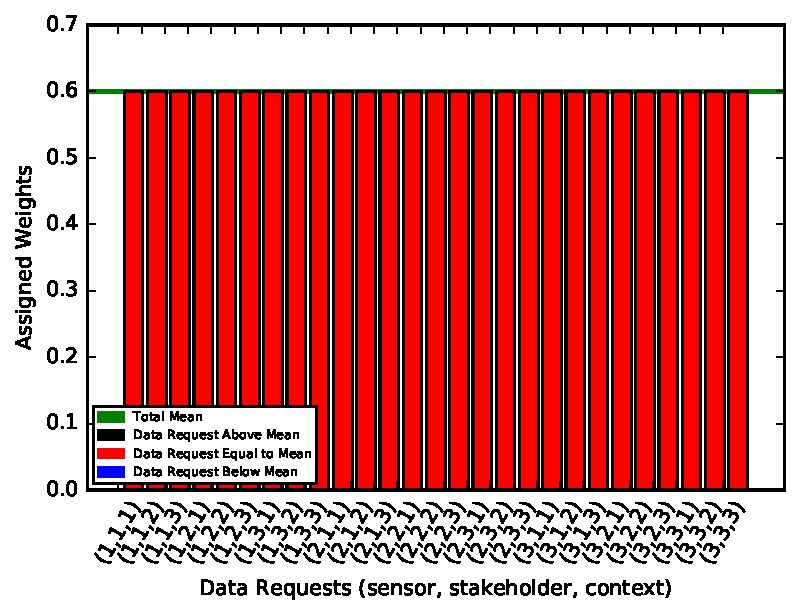
\includegraphics[width=0.5\linewidth]{./images/weight_1_1}}%
  \subtop[Values of the Cost Matrix \label{cost11}]{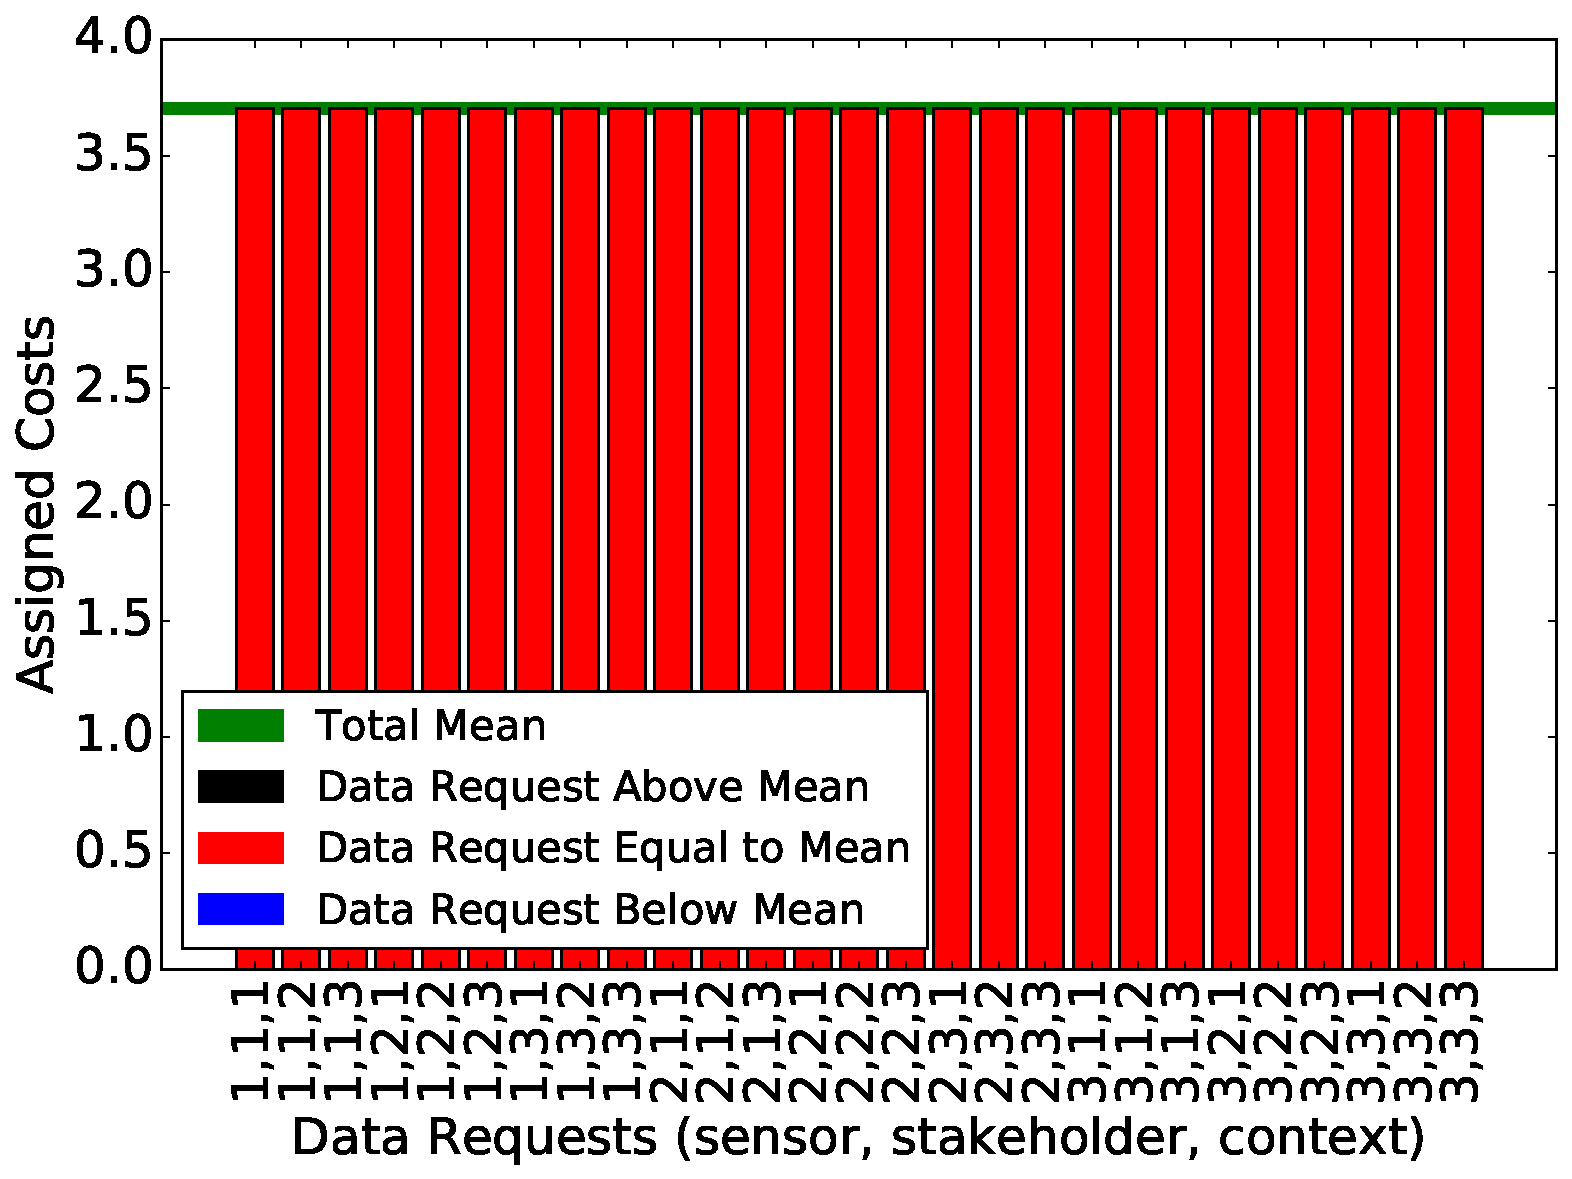
\includegraphics[width=0.5\linewidth]{./images/cost_1_1}}%
  \caption{Examining Scenario 1}
  \label{fig:scenatio11}
\end{figure}



We can conclude that if the users perceive the featur and respective sub-features in an equally intrusive way, then all the
data requests will have the same weight and costs assigned.

\subsubsection{Scenario 2}
In this section we would like to test if data requests containing sub-features with higher intrusion levels are assigned higher weights and costs.
Table \ref{tab:scenario3} indicates the user input to scenario 2. As it can be seen, all features have equal categories, and
all sub-features have the categories of 3 with an exception the  Sensor's sub-features. The Sensors sub-features with identifiers 1,2 and 3 have respectively categories 1,3 and 5. This means that requests with Sensor's sub-feature 1 will be assigned a lesser weight in comparison to the other Sensors sub-features. Similarly, the data requests
with Sensors sub-feature 2 will have a higher weightage assigned than Sensor's sub-feature 1 because of its higher category, but lesser than Sensor's sub-feature 3. Lastly, data requests with Sensor's sub-feature 3 will have a highest weight compared to the others, due to its category being 5. The weight and cost matrices can be seen in figures \ref{weight3} and \ref{cost3} respectively.

\begin{table}[h!]
  \centering
  \caption{Categorization for Scenario 2}
  \label{tab:scenario3}
  \begin{tabular}{cccc}
    \toprule
    Feature & Sub-Feature ID = 1 & Sub-Feature ID = 2 & Sub-Feature ID = 3\\
    \midrule
    Sensors & Accelerometer & Noise & Location\\
     3 & 1 & 3 & 5\\ \hhline{====}
     Stakeholders & Corporation & Government & Educational Institution\\
     3 & 3 & 3 & 3\\ \hhline{====}
     Contexts & Navigation & Environment & Social Media\\
     3 & 3 & 3 & 3\\ 
    \bottomrule
  \end{tabular}
\end{table}

\begin{figure}[htp]
  \subtop[Values of the Weight Matrix\label{weight3}]{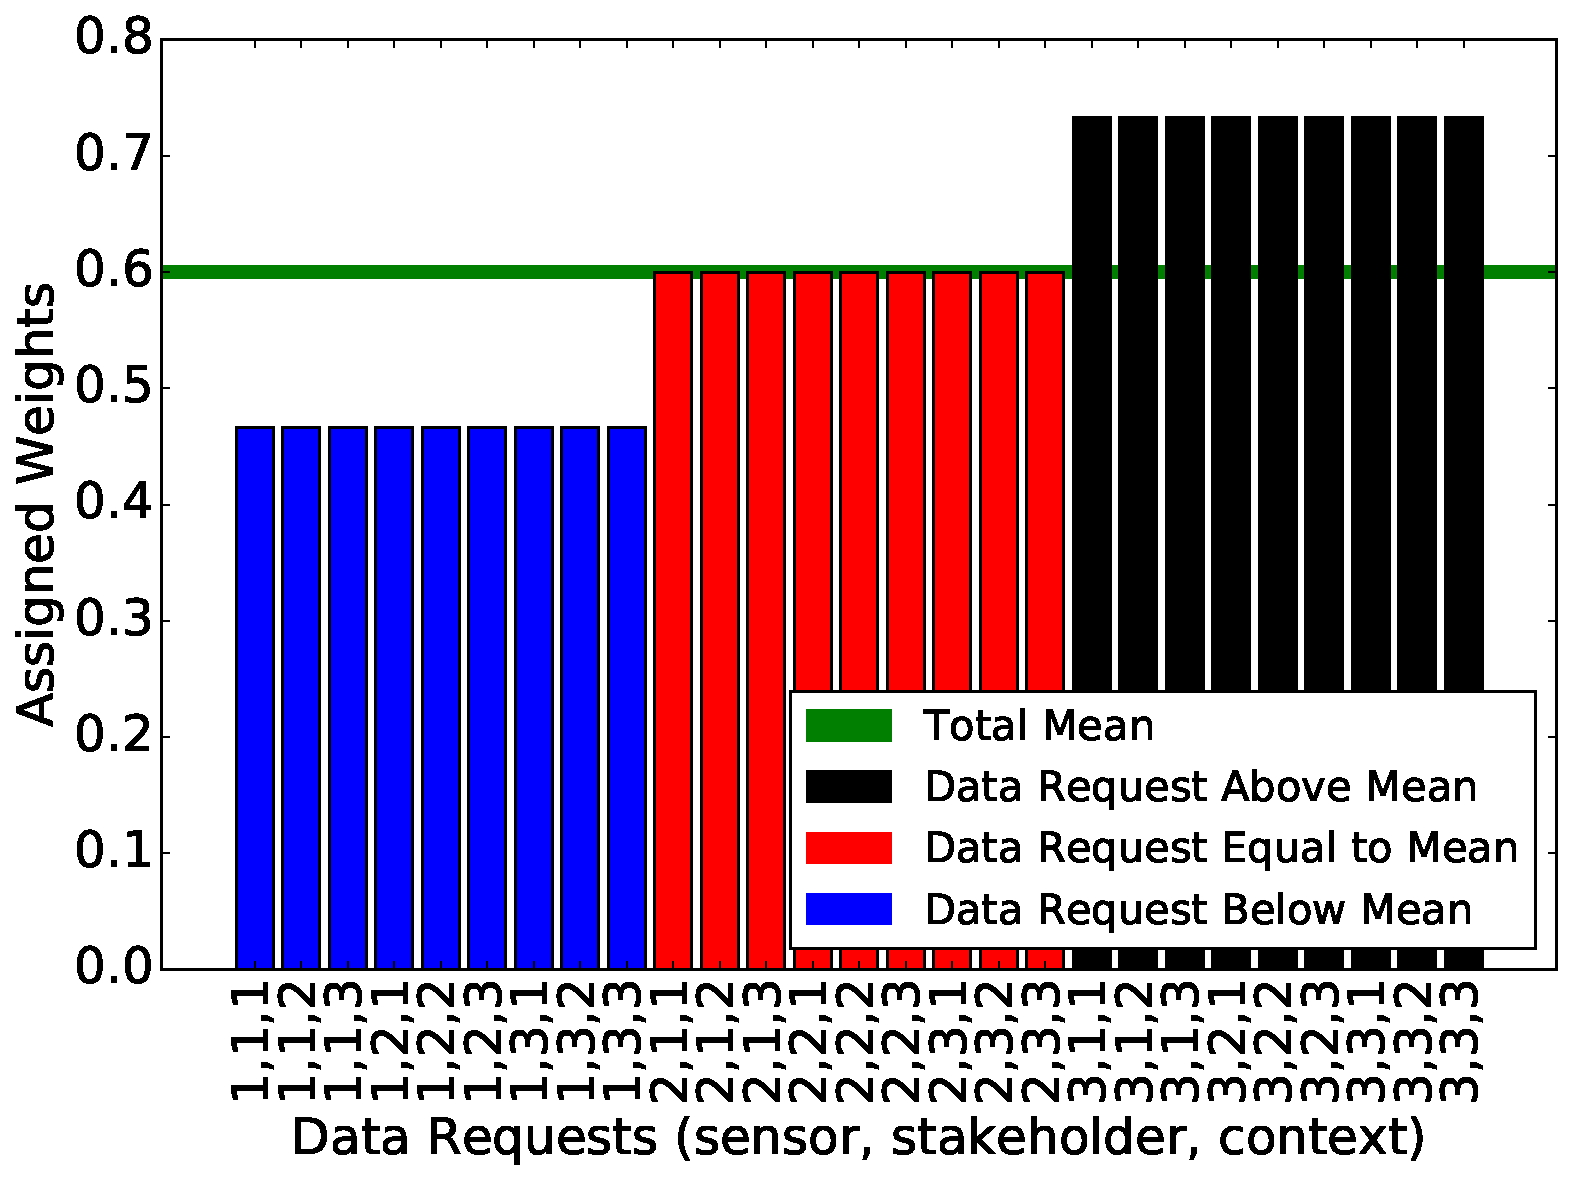
\includegraphics[width=0.5\linewidth]{./images/weight_3}}%
  \subtop[Values of the Cost Matrix \label{cost3}]{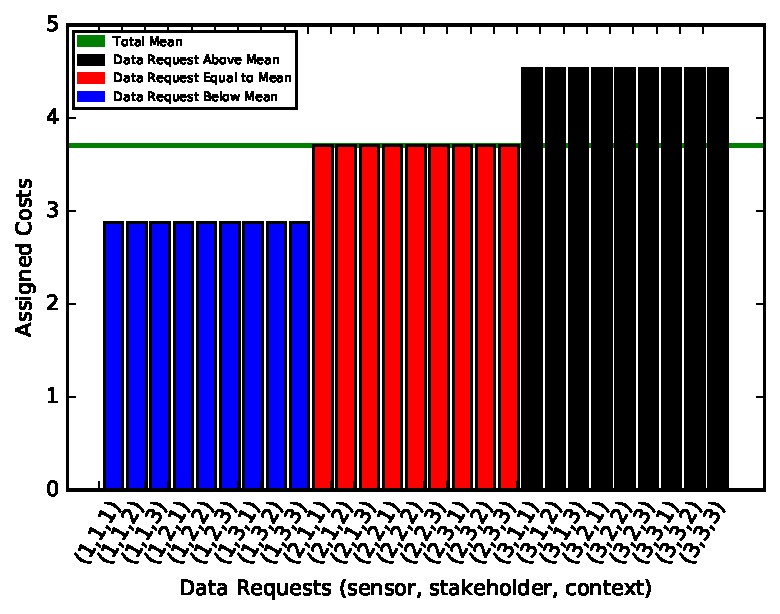
\includegraphics[width=0.5\linewidth]{./images/cost_3}}%
  \caption{Examining Scenario 2}
  \label{fig:scenatio3}
\end{figure}


From the above inputs and graphs, we can conclude that the model assigns a higher weightage to data requests with sub-features that the user finds more intrusive compared to the others.

\subsubsection{Scenario 3}
The feature and sub-feature categories are both assigned different values in this section, to show how varying their values together affects the assignments of the weight and cost matrix. Table \ref{tab:scenario4} is the user input to the scenario 3. All the features have different categories assigned from 3 to 5. Additionally, the sub-feature 1 of each feature has a category of 5, higher than the other sub-features which are all categorized as 1. The weight and cost matrices generated for this scenario can be seen in figures \ref{weight4} and \ref{cost4} respectively. 

\begin{table}[h!]
  \centering
  \caption{Categorization for Scenario 3}
  \label{tab:scenario4}
  \begin{tabular}{cccc}
    \toprule
    Feature & Sub-Feature ID = 1 & Sub-Feature ID = 2 & Sub-Feature ID = 3\\
    \midrule
    Sensors & Accelerometer & Noise & Location\\
     5 & 5 & 1 & 1\\ \hhline{====}
     Stakeholders & Corporation & Government & Educational Institution\\
     4 & 5 & 1 & 1\\ \hhline{====}
     Contexts & Navigation & Environment & Social Media\\
     3 & 5 & 1 & 1\\ 
    \bottomrule
  \end{tabular}
\end{table}

As it is observed in both figures, the data request with the highest weight is the one with tuple (1,1,1). This tuple indicates that the data request involves all sub-feature 1 of each feature. This happens because all of the sub-feature 1 are assigned a category of 5. The feature sensors and its sub-feature 1 are categorized as 5, so all the data requests
with tuple (1,*,*), where * is all the other possible sub-features from other features, are all above average as seen in figures \ref{fig:scenatio4}, irrespective of the categories of the other feature's sub-features. This shows that assigning a higher category to a feature can lead to higher data request costs. 

\begin{figure}[htp]
  \subtop[Values of the Weight Matrix\label{weight4}]{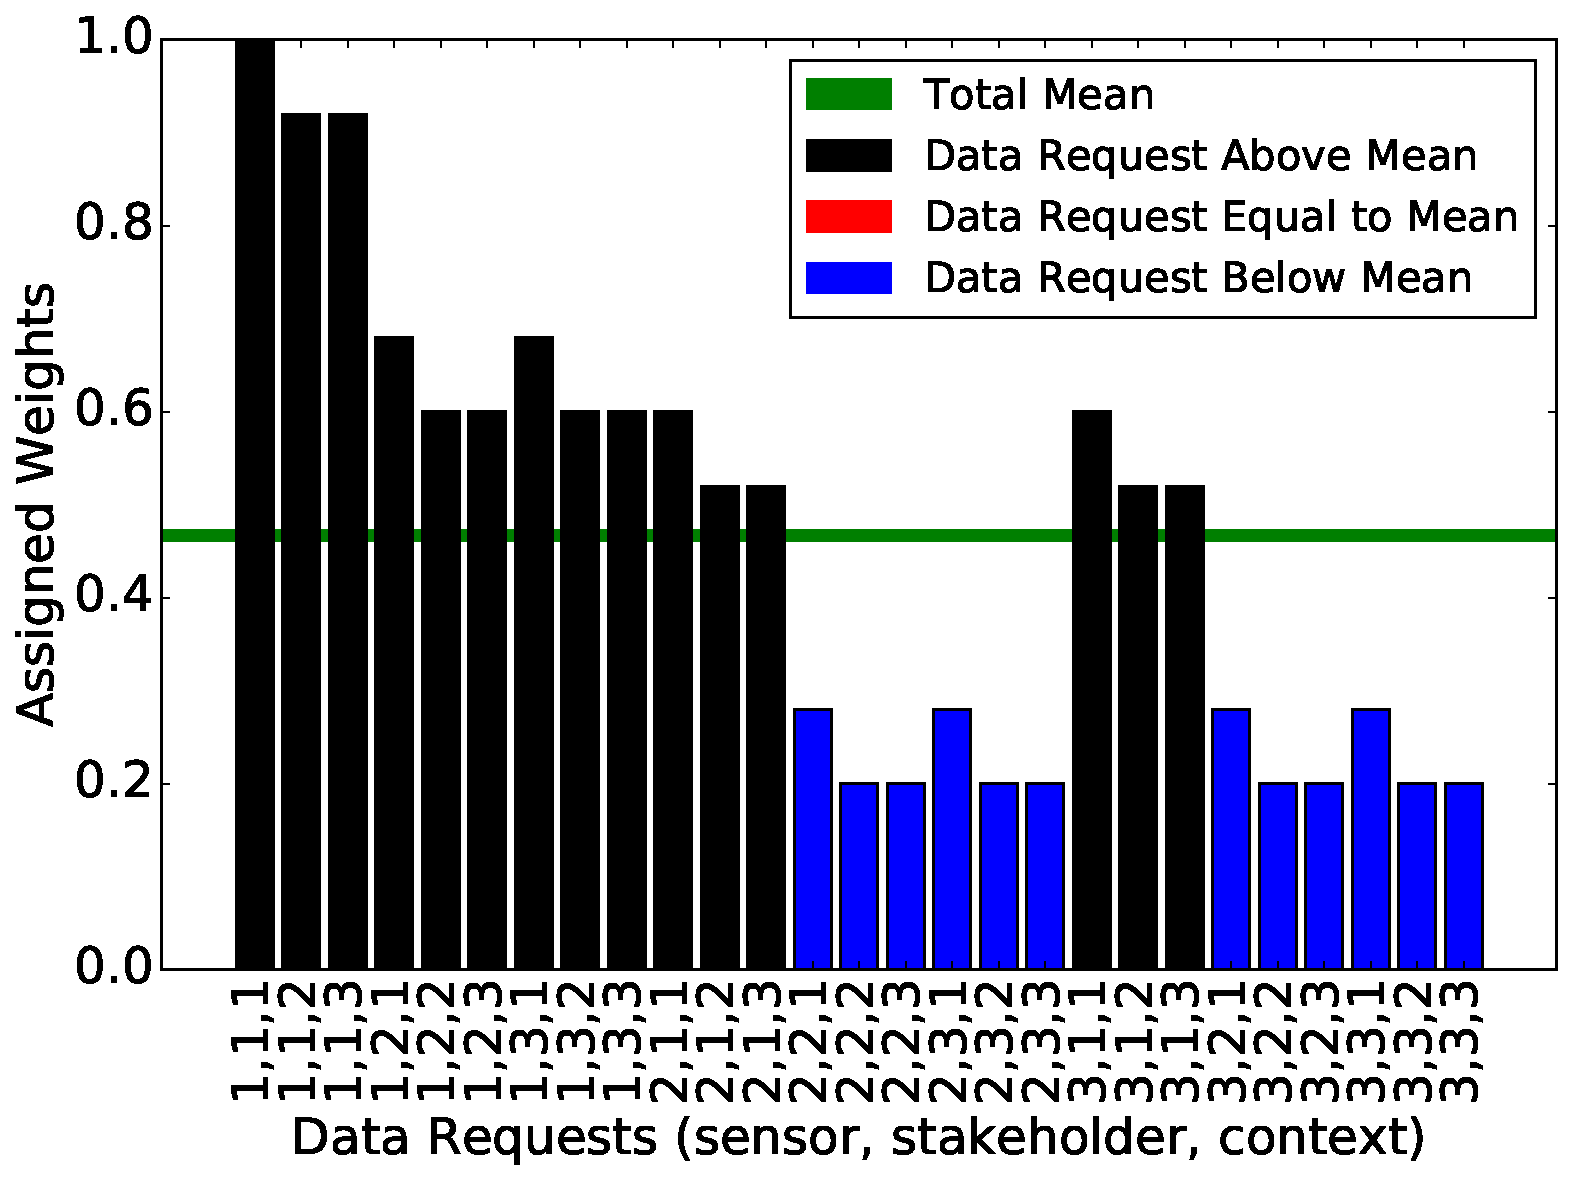
\includegraphics[width=0.5\linewidth]{./images/weight_4}}%
  \subtop[Values of the Cost Matrix \label{cost4}]{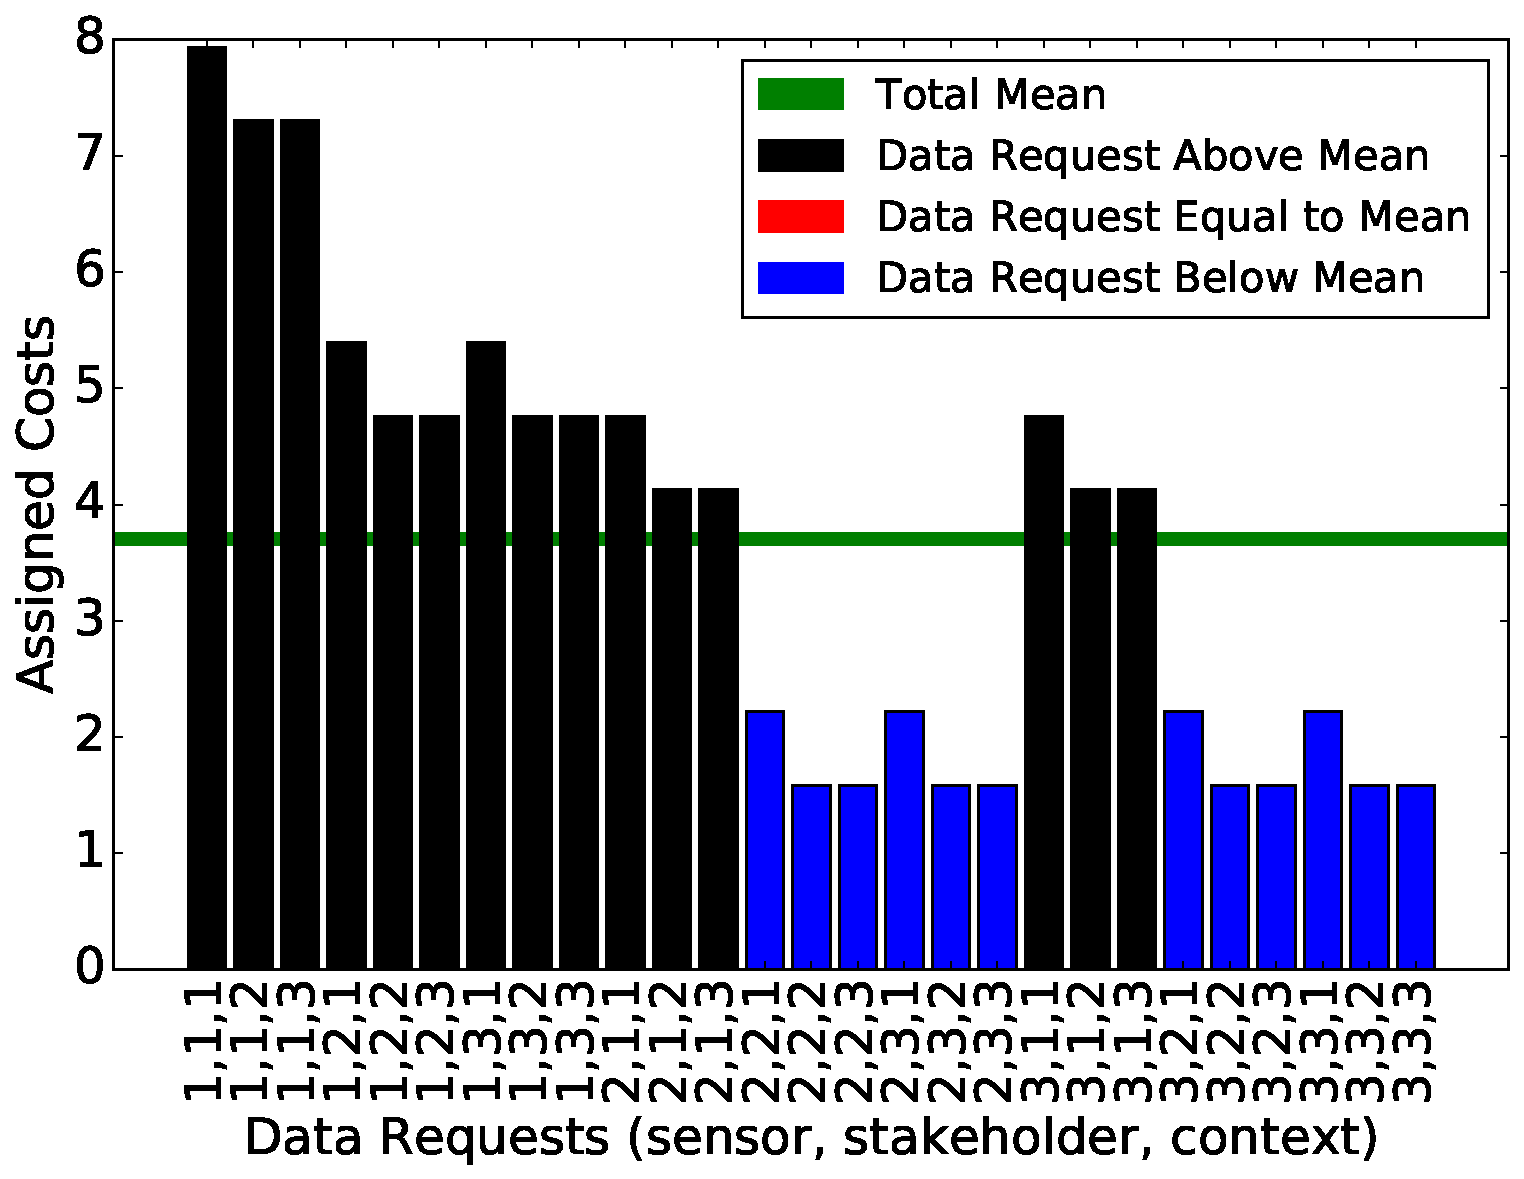
\includegraphics[width=0.5\linewidth]{./images/cost_4}}%
  \caption{Examining Scenario 3}
  \label{fig:scenatio4}
\end{figure}

The green horizontal line in the graph indicates the mean value of the weights and costs. In general due to sub-features categorized as 5, those data requests receive a higher weight and cost. In some cases, the data requests still receive a lower weight such as tuple (2,2,1),
(2,3,1),(3,2,1) and (3,3,1) even tough Contexts sub-feature 1 has a category of 5. This is due to the fact that Sensors  and Stakeholders feature have a higher category of 5 and 4 respectively than the contexts feature. Since their sub-features are assigned a lower privacy intrusion category than the context's sub-features, the weight of the data requests is lower. This shows that even tough a sub-feature may be regarded as very intrusive, it's weight increasing changing ability still depends on the category of the feature it belongs to.

Additionally, it can be noted that data requests with at least two sub-features 1 are all above average. We can witness the property of the model, which puts more emphasis on the perception of the features than the sub-features themselves. As seen in the figure, all the features with higher intrusion categorizations have weights and costs that are well above average.

It can  beconcluded that the model assigns weights to data requests, by putting more emphasis on the feature's weights. A feature with high category
has the ability to assign higher costs with a highly categorized sub-feature. It also has the ability to lower the weight of a data request with a sub-feature lowly
categorized. Features with lower categories contribute lesser to the weight assignments, irrespective of their sub-feature categories.







